\documentclass[border={0pt 0pt 0pt 0pt}]{standalone}
\usepackage{tikz} 
\usepackage{ctex}
\usepackage{CJKfntef}
\usepackage{amsmath}
\usepackage{amsthm}
\usepackage{amssymb}
\DeclareMathOperator{\Img}{\operatorname{Im}}
\definecolor{rede}{rgb}{1,0.97647,0.97647}
\definecolor{browne}{rgb}{0.619608,0.258824,0}
\usetikzlibrary{shapes.geometric, arrows, arrows.meta, fit, backgrounds, decorations.pathmorphing, petri, calc,positioning,shapes.misc,graphs}
\begin{document}
			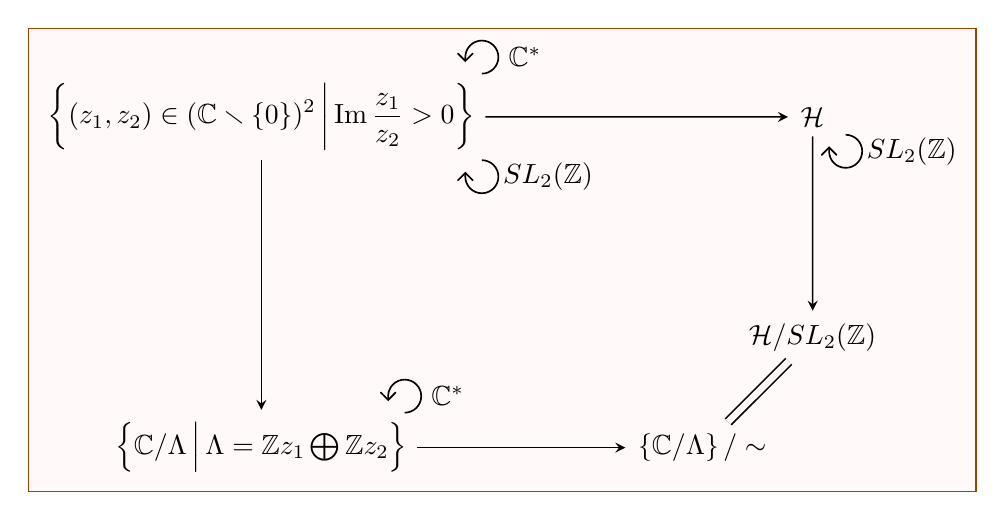
\begin{tikzpicture}[scale=1.4, ->, shorten >=1pt, >=stealth, semithick]

\node (zuoshang) at (0,3) []{$\displaystyle\left\{(z_1,z_2) \in (\mathbb{C}\smallsetminus \{0\})^2 \,\middle|\, \Img \frac{z_1}{z_2} >0\right\}$};
\node (H) at (5,3) []{$\mathcal{H}$} ;
\node (modularcurve) at (5,1) []{$\mathcal{H}/SL_2(\mathbb{Z})$};
\node (torus) at (0,0) []{$\left\{\mathbb{C}/\Lambda\, \Big|\, \Lambda=\mathbb{Z}z_1 \bigoplus \mathbb{Z}z_2 \right\}$};
\node (modular space) at (4,0) []{$\left\{\mathbb{C}/\Lambda\right\}/\sim$};
\draw [->,>=angle 90]($(zuoshang.south) + (0:2cm)$) arc 
(90:-180:1.5mm) node [right=10pt] {$SL_2(\mathbb{Z})$} -- ++(-270:2pt);
\draw [->,>=angle 90]($(zuoshang.north) + (0:2cm)$) arc 
(-90:180:1.5mm) node (1)[right=12pt] {$\mathbb{C}^*$} -- ++(270:2pt);
\draw [->,>=angle 90]($(H.south) + (0.1cm:0.3cm)$) arc 
(90:-180:1.5mm) node(2)[right=10pt] {$SL_2(\mathbb{Z})$} -- ++(-270:2pt);		
\draw [->,>=angle 90]($(torus.north) + (0:1.3cm)$) arc 
(-90:180:1.5mm) node[right=12pt] {$\mathbb{C}^*$} -- ++(270:2pt);	
\path (zuoshang) 
edge [] (H)		
edge [] (torus)
(H) edge [] (modularcurve)
(torus) edge [] (modular space)			
(modularcurve) edge [-,double=rede, double distance between line centers=0.3em] (modular space)	 ;

\begin{scope}[on background layer]
\node [draw=browne,fill=rede,fit=(zuoshang)(H)(modularcurve)(torus)(modular space)(1)(2)] {};
\end{scope}
\end{tikzpicture}

\end{document}
